\chapter{Imprecise Probability as Foundation of Generalised Bayesian Inference}
\label{cha:gbi}

%\begin{itemize}
%\item Short introduction to IP (sets of priors, lower/upper prevision/probability)
%\item motivate imprecise priors with ress paper: \cite{Troffaes2013a} --- now in intro
%\item \pdc\ (Evans \& Moshonov, Fuquene-Cook-Pericchi) somewhere???*** %, examples (Festschrift paper: \cite{Walter2010a})
%\item further motivations for IP (ITIP chapter \cite{itip-statinf}) 
%\item Generalized Bayesian inference
%\item Generalized Bayesian inference with sets of priors
% \begin{itemize}
% \item sets of priors, GBR, robust Bayes
% \item sets of conjugate priors in general
% \item parameter set shapes
% \end{itemize}
%\item IDM
%\item JSTP paper \cite{Walter2009a}
%\item isipta11 paper \cite{Walter2011a}
%\item boatshape?
%\end{itemize}



After having seen a detailed example for Bayesian inference using sets of conjugate priors in Section~\ref{sec:commoncause},
in this chapter we will now give a general introduction to the methodology of generalised Bayesian inference,
before we give a systematic discussion of models for generalised Bayesian inference with sets of conjugate priors
in the central Section~\ref{sec:generalmodel} of this thesis.

\medskip

In Section~\ref{sec:ip-intro} below, we will try to outline the general theory of imprecise or interval probability,
describing its main formulations and interpretations, and discuss the generalised Bayesian inference procedure.
Section~\ref{sec:motivation} then gives at first some general motives for the use of imprecise probability methodology,
concluding with the motives especially relevant in the context of the Bayesian approach to statistical inference,
among which prior-data conflict and weakly informative priors will receive special attention
in the model discussion in Chapter~\ref{cha:imprecisebayes-conjugate}.

%***Section~\ref{sec:alternatives} ****


\section{Imprecise or Interval Probability}
\label{sec:ip-intro}

This Section will give a condensed introduction to the main theoretic concepts
in interval or imprecise probability as needed for the topics discussed in this thesis.
Here, we take a decidedly epistemic view on interval or imprecise probability,
as we will argue in Section~\ref{sec:motivation}
that imprecise probability distributions are often a better tool for expressing prior beliefs
than precise probability distributions.

%While Section~\ref{sec:ip-general} follows mostly \textcite{2011:IESS-ip},
%Section~\ref{sec:ip-main} is based mainly on \textcite{1996:walley::expert} and \textcite{2000:walley::towards}.


\subsection{General Concept and Basic Interpretation}
\label{sec:ip-general}

The central idea of imprecise or interval probability \parencite{1991:walley, 2001:weichselberger, 2011:IESS-ip} is
to replace the usual, precise probability measure $\p(A)$ for events $A$%
\footnote{Events of interest $A$ are taken to be subsets of the sample space $\Omega$,
forming a $\sigma$-algebra, a non-empty collection of sets including countable unions and intersections of subsets of $\Omega$.}
with a \emph{lower} and \emph{upper probability}, denoted by $\Pl(A)$ and $\Pu(A)$, respectively,
satisfying
\begin{equation}
\label{eq:0ip1}
0 \le \Pl(A) \le \Pu(A) \le 1\,.
\end{equation}
In this setting, a usual probability measure forms the extreme case $\Pl(A) = \Pu(A) = \p(A)$,
when there is enough information to determine the distribution on the sample space $\Omega$
in precise stochastic terms.
On the other extreme, when $\Pl(A) = 0$ and $\Pu(A) = 1$,
we have no information at all on the probability for $A$ to occur,
and intermediate cases $0 \le \Pl(A) < \Pu(A) \le 1$ represent
different degrees of knowledge on this probability.

Therefore, interval or imprecise probability adds another modeling dimension:
While usual, precise probability measures can be used to model phenomena when there is perfect stochastical information,
like, e.g., in a lottery where the number of winning tickets (and the total number of tickets) is precisely known,
imprecise probability measures can account for cases where there is uncertainty about the probabilities themselves,
just like in a lottery where the number of winning tickets is not exactly known.
Non-stochastic uncertainty about model features like probabilities is often called \emph{ambiguity},%
\footnote{See Section~\ref{sec:motivation-riskambiguity}.}
forming a crucial part of the human decision process,
and there are studies suggesting that humans process ambiguity in a way
differing from pure probabilistic reasoning \parencite{2005:hsu-bhatt}.

In contrast to a probability measure $\p(A)$,
the set functions $\Pl(A)$ and $\Pu(A)$ do not adhere
to the additivity axiom of Kolmogorov's \parencite*{1933:kolmogorov}
formalisation of probability as a normed measure,
%(countable or finite additivity),
and thus are also known as \emph{non-additive probabilities}.
There is also a link to \emph{fuzzy measures}, which are also non-additive measures
\parencite[see, e.g.,][]{1997:denneberg}.

In general, $\Pl(A)$ may be understood as accounting for evidence certainly in favour of $A$,
and $\Pu(A)$ accounting for all evidence speaking not strictly against $A$.
The difference of $\Pu(A)$ and $\Pl(A)$ thus allows for inconclusive evidence
that may not speak unanimously in favor of or against $A$, respectively.
As evidence strictly against $A$ can be seen as evidence certainly in favour of $A^\com$,
the complement of $A$,
it is mostly assumed that $\Pl(A^\com) = 1 - \Pu(A)$,
and thus it suffices to determine either of $\Pl$ or $\Pu$,
the other one being defined through this relation.

There are currently two main approaches to a general theory of statistical inference with interval or imprecise probability:
\begin{enumerate}[(i)]
\item The theory by Weichselberger \parencite*{2000:weichselberger, 2001:weichselberger}
regards probability intervals $[\Pl(A), \Pu(A)]$ for all or some events $A$ as the basic entity
\parencite[p.~646]{2011:IESS-ip},
from which an interval-valued distribution on the sample space $\Omega$ is constructed.
His approach is axiomatic, in the sense that it replaces Kolmogorov's \parencite*{1933:kolmogorov} additivity axiom by two axioms,%
\footnote{The first states that \eqref{eq:0ip1} holds,
the second that the set $\mathcal{M}$ consisting of all usual, precise distributions $\p(\cdot)$
with $\Pl(A) \le \p(A) \le \Pu(A)$, for all $A \in \Omega$, is non-empty.
The second axiom guarantees that there exists at least one precise probability distribution
which is compatible with an interval-valued probability distribution,
and thus rules out the case of contradictory assignments of $[\Pl(A), \Pu(A)]$.}
from which the theory is derived,
while imposing no specific interpretation on these constructs.
This theory of interval probability was developed
as the foundation of a concept of \emph{logical probability} \parencite{2007:weichselberger},
where probability is not assigned to events, but to logical conclusions (from a premise to a consequence),
with the aim to arrive at a theory of statistical inference
which allows for fiducial-like probability statements,
e.g., probability statements on parameters similar to those derived from a posterior distribution in a Bayesian setting,
but without the need to specify a prior distribution \parencite[see, e.g.,][]{2011:IESS-fiducial}.
\item In contrast, the theory by Walley \parencite*{1991:walley, 2000:walley::towards}
aims to generalise the Bayesian approach to statistical inference,
adopting a strictly subjective, behavioural interpretation for imprecise probability
as lower and upper betting rates (see below),
and extending the Bayesian inference paradigm (as discussed in Section~\ref{sec:bayes-inference})
to imprecise probability distributions.
In generalising de Finetti \parencite*{1937:finetti,1970:finetti}, the basic entities are lower and upper \emph{previsions},
i.e.\ expectation functionals, for \emph{gambles}, i.e.\ random quantities,
instead of lower and upper probabilities for events.
This is due to the fact that unlike in the theory of precise probability%
---where the definition of a distribution via expectations %precise previsions
(often denoted \emph{linear previsions} in the imprecise probability literature)
is eqivalent to a definition via a precise probability distribution---%
the definition of an imprecise distribution via lower and upper previsions
is more general than a definition via lower and upper probability for events
\parencite[p.~132]{2000:walley::towards}.
\end{enumerate}
As this thesis is concerned with a generalisation of Bayesian inference
based on sets of conjugate priors, the approach by Walley,
and its reliance on a subjective, epistemic interpretation of (imprecise) probability
as (bounds for) betting rates, is now described in more detail.


\subsection{Main Formulations}
\label{sec:ip-main}

%lower and upper probabilities or expectations,
%link to sets of probability distributions,
%sets of desirable gambles as mathematical formulation,
%lower and upper betting rates,
%inference procedure (itip)

The main mathematical formulations for imprecise distributions
in the theory by Walley \parencite*{1991:walley, 2000:walley::towards}
are
\begin{enumerate}[(i)]
\item lower previsions,
\item sets of (precise) probability distributions, and
\item sets of desirable gambles.
\end{enumerate}
It is possible to switch between these formulations,
although (ii) can be slightly more general than (i),
and to a greater extent, (iii) is more general than (ii) \parencite{2000:walley::towards}.

\medskip

We will first introduce lower previsions
and the most important rationality requirements guiding their assessment and use,
then have a brief look at sets of desirable gambles as the most comprehensive formulation.
Sets of probability distributions, as the formulation used to describe inference models in this thesis,
are then explained in relation to the other formulations,
and the generalised Bayesian inference procedure as used in Section~\ref{sec:imprecise-alpha} is justified formally.

\subsubsection{Lower Previsions}
\label{sec:lowerprevisions}

As mentioned in Section~\ref{sec:ip-general}, the basic entities in the theory by \textcite{1991:walley}
are lower and upper \emph{previsions}.
These are functions on \emph{gambles}, or \emph{random variables},
defined as bounded mappings from $\Omega$ to $\reals$.
A gamble $X$ can be understood as uncertain reward or payout,
where the reward $X(\omega)$ depends on $\omega \in \Omega$,
the unknown `state of the world' from the possibility space $\Omega$.
The reward is measured in units of utility assumed to form a linear scale
\parencite[\S 2.2]{1991:walley}.

A \emph{lower prevision} or \emph{lower expectation} is then a mapping
$\El: \mathcal{K} \to \reals$, where $\mathcal{K}$ is a set of gambles.%
\footnote{In Walley's central monography \parencite{1991:walley},
his papers and the imprecise probability literature in general,
lower previsions are usually denoted by $\Pl$.
Furthermore, events $A \subset \Omega$ are notationally identified with the
indicator function $I_A(\omega)$, being a gamble with payout $1$ if $\omega \in A$ and else $0$,
such that $\Pl(A)$ denotes the lower probability of $A$.
In order to follow conventions in statistical literature, however,
lower previsions are denoted by $\El$ here,
and $\Pl$ refers exclusively to lower probabilities.}
Central to Walley's theory is the interpretation of $\El[X]$
as the subject's supremum buying price for $X$, that is,
the subject is disposed to pay at most the fixed amount $\El[X]$
in exchange for the uncertain reward $X$.%
\footnote{More precisely, the price the subject is disposed to pay for $X$ is strictly less than $\El[X]$.
For sake of readability,
this mathematically important distinction is not rigorously maintained in this brief treatment,
as it is hardly relevant for the interpretation of the results in the later parts of this thesis.}
$\El[X]$ thus expresses the subject's state of knowledge about the value of $X$,
factoring in the propensity of all possible $\omega \in \Omega$
with their specific payouts $X(\omega)$.
The \emph{upper prevision} $\Eu[X]$ is the infimum selling price for $X$,
i.e., the fixed amount the subject is willing to receive in exchange for $X$
\parencite[p.~9]{1996:walley::expert}.
Walley's theory is based on this behavioral, epistemic interpretation of previsions,
%\parencite[Section~4]{1996:walley::expert},
and all rationality criteria and inference procedures
are deduced from this root \parencite[p.~5]{1996:walley::expert}.

The theory allows thus a zone of indeterminacy, by $\El[X] < \Eu[X]$,
for prices of $X$ at which the subject is neither willing to buy nor to sell the gamble $X$,
as illustrated in Figure~\ref{fig:pricesforgambles}.
This is in contrast to the usual epistemic operationalisation of subjective Bayesian probability,
which implies that $\El[X]$ and $\Eu[X]$ must coincide at a unique fair price $\E[X]$.
This requirement is refuted by Walley, and called by him \emph{the Bayesian dogma of precision}
\parencite[\S 5]{1991:walley}.

\begin{figure}
\centering
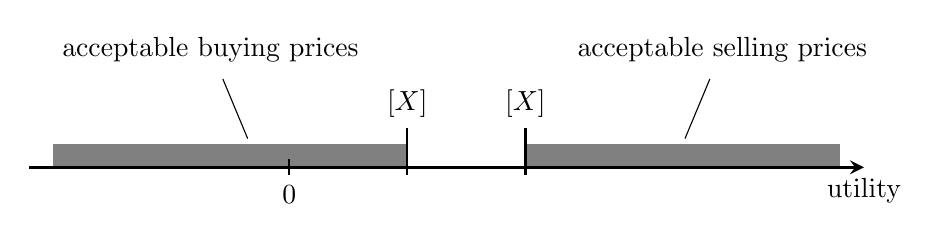
\begin{tikzpicture}[%
linkline/.style={
  shorten >= 2pt,
  shorten <= 3pt
}%
]
\path[fill=gray] (0,0) rectangle (4.5,0.3);
\path[fill=gray] (6,0) rectangle (10,0.3);
\draw[very thick,-stealth] (-0.3,0) -- (10.3,0) node[below] {utility};
\draw[thick] (3,0.1) -- (3,-0.1) node[below] {$0$};
\draw[thick] (4.5,-0.1) -- (4.5,0.5) node[above] {$\El[X]$};
\draw[thick] (6,-0.1) -- (6,0.5) node[above] {$\Eu[X]$};
\node (buy) at (2,1.5) {acceptable buying prices};
\node (sell) at (8.5,1.5) {acceptable selling prices};
\draw[linkline] (buy) -- (2.5,0.3);
\draw[linkline] (sell) -- (8,0.3);
\end{tikzpicture}
\caption[Illustration of \underline{E}\ and $\Eu$ as supremum buying and infimum selling prices]{\label{fig:pricesforgambles}%
Illustration of \underline{E}\ and $\Eu$ as supremum buying and infimum selling prices for a gamble $X$ on a linear utility scale.}
%$\El$ %strange errors occur
\end{figure}

A lower and upper prevision are called \emph{conjugate}%
\footnote{Conjugacy in this sense should not be confused
with conjugacy for prior distributions as discussed in Section~\ref{sec:regularconjugates}.}
if the relation $\Eu[X] = -\El[-X]$ holds for all $X \in \mathcal{K}$.%
\footnote{This implies the relation $\Pl(A^\com) = 1 - \Pu(A)$
of lower and upper probabilities for events $A \subset \Omega$
as mentioned in Section~\ref{sec:ip-general}.}
Then, it suffices to consider only either of $\El$ or $\Eu$,
and in the literature $\El$ is chosen,
the theory consequently being referred to as the theory of
\emph{coherent lower previsions} \parencite[see, e.g.,][\S 3.2]{itip}.

\subsubsection{Coherence and Avoiding Sure Loss}

Before we come to the concept of \emph{coherence},
a weaker rationality requirement put forward by Walley is
that a lower prevision $\El$ should fulfill the property of
\emph{avoiding sure loss} \parencite[\S 2.4]{1991:walley}.
This means that a subject, whose state of information about the
occurrence of `states of the world' from the possibility space $\Omega$
is encoded in his or her choice of $\El$,
acting by buying and selling gambles accordingly,
should choose $\El$ such that there is no combination of gambles
%$X_i$, $i=1,\ldots,k$, %of which each is, by $\El$, 
that would result in a net loss, whatever $\omega \in \Omega$.
As an analogy, \emph{avoiding sure loss} can be regarded
like a logical inconsistency in a set of propositions,
i.e., there exist two propositions in the set of propositions
(the analogy to $\El$) which are contradictory
\parencite[\S 2.4, footnote~1]{1991:walley}.

Continuing this analogy, $\El$ violating the stronger property of \emph{coherence}
is like the ``failure to deduce all [\ldots] logical implications''
\parencite[\S 2.4, footnote~1]{1991:walley} from the set of propositions.
As an example, if a subject assesses $\El$ such that $\El[X] = \El[Y] = \frac{1}{4}$,
and also that $\El[X+Y] = \frac{1}{4}$, $\El$ avoids sure loss, but is not coherent,
because one can imply from $\El[X] = \El[Y] = \frac{1}{4}$ that
$\El[X+Y]$ must be at least $\frac{1}{2}$ \parencite[p.~67]{1991:walley}.
Coherence is a ``normative requirement of consistency'' \parencite[p.~130]{2000:walley::towards}
that is a consequence of few basic rationality requirements.
In fact, if $\mathcal{K}$ is a linear space of gambles,
i.e., $\mathcal{K}$ is closed with respect to addition and multiplication with constants,
then coherence is equivalent to the three following conditions
\parencite[e.g.,][p.~11]{1996:walley::expert}:
\begin{enumerate}[(i)]
\item $\El[X] \ge \inf_{\omega \in \Omega} X(\omega)$,
i.e., one is always prepared to buy a gamble for less than its minimum possible reward.
(Being prepared to pay more than $\inf_{\omega \in \Omega} X(\omega)$ amounts to making a commitment to the
possibility that other states $\omega'$ with $X(\omega') > \inf_{\omega \in \Omega} X(\omega)$ may occur.)
\item $\El[\lambda X] = \lambda \El[X]$ for all $X \in \mathcal{K}$, $\lambda > 0$.
$\El$ should be such that if it postulates that one should be prepared to buy a gamble $X$ at a price
of at most $\El[X]$, then one should also buy gambles that are fractions or multiples of $X$
at prices of at most the original price divided or multiplied accordingly.
This illustrates that prices are to be understood on a linear utility scale
(as mentioned above) and should not be considered as plain monetary prices,
for which this condition may not be reasonable.
\item $\El[X+Y] \ge \El[X] + \El[Y]$.
This property of superlinearity or superadditivity implies that the supremum acceptable buying price for $X$ and $Y$ combined
should be at least the sum of supremum acceptable buying prices for each of $X$ and $Y$ individually.
It could be, e.g., that $X$ and $Y$ balance out each other in a way that
buying both of them at once makes the transaction less risky,
such that a higher price limit for $X + Y$ is acceptable.
Usual precise expectations, for which additivity $\E[X+Y] = \E[X] + \E[Y]$ must hold,
cannot directly accommodate such reasoning.
\end{enumerate}

Consequently, in analogy to deducing all logical implications from
a set of propositions, there is a technique, %for lower previsions,
called \emph{natural extension}, that adjusts
a given assessment of lower and upper previsions (on some set of gambles $\mathcal{K}$, which must avoid sure loss)
to make it coherent, in the least committal way as possible%
\footnote{This means that there may be other adjustments of $\El$ that are compatible
with the initial assessments, but are less conservative,
i.e., give higher supremum buying prices.}
\parencite[see, e.g.,][pp.~15ff]{1996:walley::expert}.
This is accomplished by a linear program,
and may involve raising $\El[X]$ for some $X \in \mathcal{K}$ in order to make them
coherent to the values of $\El[Y]$, supremum buying prices for some other gambles $Y \in \mathcal{K}$ as previously assessed,
or newly defining $\El[Z]$ for gambles $Z$ not considered during assessment---explaining the name `extension'.

\subsubsection{Sets of Desirable Gambles}

Sets of desirable gambles \parencites[\S 6]{2000:walley::towards}{itip-desirable} are an alternative formulation
for probability assessments as expressed by a lower prevision $\El$.
They are a mathematically convenient formulation
and as such a very useful tool in the development of the theory of imprecise probability.
However, a detailed understanding of this concept is not necessary for the purpose of this thesis,
and the account below is intended to give some insight into this central concept in the theory of imprecise probability.

The \emph{gambles} here are again a description of an uncertain reward as above, 
and all bounded functions from $\Omega$ to $\reals$
are forming the space $\mathcal{L}$ of all gambles.
The assessment in this formulation lies in the designation of a subset $\mathcal{D}$
of all gambles $\mathcal{L}$ as \emph{desirable gambles},
i.e., as supplying an uncertain reward (in utilities) for which,
from the subject's state of information
about the propensity of occurence of the different $\omega \in \Omega$,
the potential benefits outweigh the potential losses.
Thus, all gambles $X$ that will never incur a loss,
$\{X: X \ge 0\}$, where $X \ge 0$ denotes that $X(\omega) \ge 0\ \forall \omega \in \Omega$,
should be contained in a coherent set of desirable gambles $\mathcal{D}$.
Indeed, the notion of \emph{coherence} for lower previsions translates to sets of desirable gambles as follows:
$\mathcal{D} \subset \mathcal{L}$ is coherent if and only if
\parencite[p.~137]{2000:walley::towards}
\begin{enumerate}[(D1)]
\item $0 \notin \mathcal{D}$ ($0$ is the gamble $X$ with $X(\omega) = 0\ \forall \omega \in \Omega$),
\item if $X \in \mathcal{L}$ and $X > 0$ then $X \in \mathcal{D}$\\
($X > 0$ denotes that $X \ge 0$ and $\exists \omega \in \Omega: X(\omega) > 0$),
\item if $X \in \mathcal{D}$ and $c \in \posreals$ then $cX \in \mathcal{D}$,
\item if $X \in \mathcal{D}$ and $Y \in \mathcal{D}$ then $X+Y \in \mathcal{D}$.
\end{enumerate}
In $\mathcal{L}$, a coherent set of gambles $\mathcal{D}$ is thus a convex cone
containing all positive gambles $\{X: X > 0\}$ but not the zero gamble.%
\footnote{As the weaker property, a set of gambles $\mathcal{D}$ avoids sure loss
if $\posi(\mathcal{D}) \cap \{X: X(\omega) < 0\ \forall \omega \in \Omega\} = \emptyset$.
Here, $\posi(\mathcal{D}) := \{ \sum_{i=1}^n c_i X_i : c_i \in \posreals, X_i \in \mathcal{D}, n \in \naturals \}$
is the positive hull of $\mathcal{D}$, 
i.e.\ the set of gambles resulting from application of (D3) and (D4) on $\mathcal{D}$.}

A coherent set of desirable gambles can be derived from a coherent lower prevision $\El$ by
\parencite[p.~139]{2000:walley::towards}
\begin{align*}
\mathcal{D} = \left\{ X \in \mathcal{L} :
X > \sum_{i=1}^n c_i (X_i - \El[X_i] + \epsilon) \text{ for some } n \in \naturals, c_i > 0, \epsilon > 0, X_i \in \mathcal{L} \right\}\,.
\end{align*}
If we adopt $\El$ as the lower prevision expressing our beliefs about $\Omega$,
gambles $X_i - \El[X_i] + \epsilon$ should be desirabe for us;
considering the price $\El[X_i]$ as the supremum acceptable buying price for $X_i$,
the gamble $X_i - \El[X_i]$ should---in our view---be at least as good as the zero gamble.

Conversely, a coherent lower prevision can be deduced from a coherent set of desirable gambles by
$\El[X] := \sup\{c: X - c \in \mathcal{D}\}$.
%\parencite[p.~139]{2000:walley::towards}
If we make $c$ as large as possible such that the gamble $X-c$ is still acceptable to us,
then $\El[X]$ simply is our supremum acceptable buying price for $X$.

As already mentioned, sets of desirable gambles are a more general formulation
as compared to lower previsions, illustrated by the fact that there can be
several sets $\mathcal{D}$ leading to the same $\El$ \parencite[p.~139]{2000:walley::towards}.%
\footnote{Another formulation equivalent to sets of desirable gambles is the description as \emph{partial preference orderings},
where a partial ordering of the gambles in $\mathcal{L}$ is given to express beliefs on $\Omega$
\parencite[p.~138]{2000:walley::towards}.}

\subsubsection{Sets of Probability Distributions}

We now turn to the formulation of imprecise probability assessments
applied in this thesis, 
sets of (precise) probability distributions,
which are also called \emph{credal sets} \parencite[e.g.,][p.~136]{2000:walley::towards}.

There is a one-to-one correspondence between coherent lower previsions
and non-empty, closed and convex sets of (precise) probability distributions
\parencite[\S 3.6.1]{1991:walley}.
When dropping the conditions of convexity and closure,
sets of probability distributions can be slightly more general
than coherent lower previsions \parencite[\S 5]{2000:walley::towards}.
However, the nature of this slight increase in generality is not relevant here,
although we will consider the question of convexity more closely later.

Given a coherent lower prevision $\El$,
the corresponding set of distributions $\mathcal{M}$
is closed and convex, and consists of all probability distributions
whose expectations $\E_p$ dominate $\El$, i.e.,%
\footnote{The probability distributions contained in a credal set $\mathcal{M}$
will be referred to by their probability density or mass functions $p(\cdot)$
in place of their probability measures $\p(\cdot)$, as we will consider mostly the densities
in our later discussions***.}
\begin{align*}
\mathcal{M} &= \{ p(\omega) : \E_p[X] \ge \El[X]\ \forall X \in \mathcal{L}\}\,.
\end{align*}
In fact, for all $p \in \mathcal{M}$ and $X \in \mathcal{L}$,
the relation $\El[X] \le \E_p[X] \le \Eu[X]$ holds;
the set $\mathcal{M}$ consists of all probability distributions
whose expectations are compatible with the bounds defined by
the lower prevision $\El$ and its conjugate upper prevision $\Eu$.

Conversely, given a non-empty set of probability distributions $\mathcal{M}$,
where $\mathcal{M}$ needs not necessarily be closed or convex,
the corresponding coherent lower prevision, for any gamble $X \in \mathcal{L}$,
is defined by
\begin{align*}
\El[X] &= \inf_{p \in \mathcal{M}} \E_p[X]\,,
\end{align*}
and in this case, $\El$ is called the \emph{lower envelope} of $\E_p$, $p \in \mathcal{M}$
\parencite[p.~132]{1991:walley}.

There are very important relations between the notions of avoiding sure loss and coherence on the one hand,
and the formulation of imprecise probability assessments via sets of probability distributions on the other hand.
The two equivalences below are known as the \emph{lower envelope theorem} \parencite[\S 3.3.3]{1991:walley}.
\begin{enumerate}[(a)]
\item $\El$ avoids sure loss if and only if the corresponding set $\mathcal{M}$ is non-empty.
Thus, an assessment $\El$ for which there is no compatible probability distribution
must incur a sure loss, and cannot be considered as reasonable.
On the contrary, any imprecise probability distribution defined by assigning
a set $\mathcal{M}$ of probability distributions avoids sure loss.
\item Furthermore, $\El$ is coherent if and only if it can be
described as the lower envelope based on its corresponding $\mathcal{M}$.
Therefore, all coherent lower previsions are characterised as
lower envelopes based on some set of precise distributions $\mathcal{M}$,
and imprecise probability assignments established via such a set $\mathcal{M}$
are, by design, coherent.
\end{enumerate}

Although the one-to-one correspondence mentioned above holds only for closed and convex sets $\mathcal{M}$,
there is nothing in the theory preventing us to consider
open or non-convex sets $\mathcal{M}$ as our probability model, %the initial assessment,
because lower and upper previsions derived from $\mathcal{M}$ are nevertheless coherent.

%link to lower previsions, convexity
%
%lower envelope theorem: itip Prop.~3.7, p.~58, 1991:walley Prop.~3.3.3
%
%itip sec.3.2.2, 3.3.3

\subsubsection{Conditioning and the Generalised Bayes' Rule}
\label{sec:gbr}

To use imprecise probability distributions for statistical inference
in the same way as usual Bayesian inference employs precise probability distributions,
we need a notion of \emph{conditioning} or \emph{updating} for imprecise probability distributions.
In analogy to the procedure described in Section~\ref{sec:bayes-inference},
the objective is to express prior knowledge on a parameter of interest $\vartheta$
by an imprecise prior distribution,
and all inferences shall be based on the (imprecise) posterior distribution derived from it.
As in Bayesian inference with precise distributions,
the now imprecise prior should be conditioned on the observed data $\x$.

A coherent lower prevision can be conditioned on an event $B$
by using the so-called \emph{Generalised Bayes' Rule} \parencite[GBR,][\S 6.4]{1991:walley},
by which the conditional coherent lower prevision $\El[X\mid B]$
based on a lower prevision $\El[X]$ can be derived.
$\El[X\mid B]$ is then also coherent to $\El[X]$, i.e.,
it is a model satisfying the rationality criteria as discussed for $\El[X]$
now also for the beliefs expressed in $\El[X]$ contingent on $B$.%
\footnote{The adequacy of the Generalised Bayes' Rule for statistical inference procedures has been questioned in the literature,
and there is doubt that it may reasonably represent learning.
We will comment on this topic in Section~\ref{sec:updating}.}

In the formulation via a credal set, the Generalised Bayes' Rule
is equivalent to conditioning each distribution in the credal set on $B$ via Bayes' Rule
\parencite[\S 6.4.2]{1991:walley},
and the set of conditioned distributions is thus an equivalent model for $\El[X\mid B]$.
This important result is known as the \emph{lower envelope theorem for conditional previsions}.

%GBR: coherence of prior and posterior

\subsection{Generalised Bayesian Inference Procedure}
\label{sec:imprecisebayes}

%paragraph from itip

Walley has thus established a general framework for coherent statistical inference under imprecise probabilities.
It allows to transfer the basic aspects of traditional Bayesian inference to the generalised setting,
as the fundamental paradigms of Bayesian inference as discussed in Section~\ref{sec:bayes-inference} are maintained.
Prior knowledge on the parameter, expressed by a now imprecise prior distribution $\El(\cdot)$ with credal set $\mathcal{M}$,
is updated in the light of the observed sample $\x$ to the posterior $\El(\cdot \mid \x)$,
with the credal set $\mathcal{M}_{\vert \x}$,
and this statistical inference is again understood as a deductive process,
obtained directly by conditioning on the observed sample,
now according to the Generalized Bayes' Rule that ensures coherence of this inferential process.
For practical implementation of the Generalized Bayes' Rule, the lower envelope theorem for conditional 
previsions mentioned above %\parencite[\S~6.4.2]{1991:walley}
is of particular relevance.
The prior credal set $\mathcal{M}$ is updated element by element to obtain the posterior credal set %$\mathcal{M}_{\vert \mbf{x}}$
\begin{align}
\label{eq:posteriorcredalset}
\mathcal{M}_{\vert \x} = \left\{ p(\cdot \mid \x) :  p(\cdot) \in \mathcal{M} \right\}\,,
\end{align}
consisting of all posterior distributions (represented by their density or mass functions $p(\cdot \mid \x)$)
obtained by traditional Bayesian updating of elements of the prior credal set.

\subsubsection{Relation to Bayesian Sensitivity Analysis}
\label{sec:bayesiansensitivity}

Walley's lower envelope theorem also establishes a close connection to robust Bayesian approaches and Bayesian sensitivity analysis
\parencite[see, e.g.,][]{1994:berger, 2000:rios, 2005:ruggeri} based on sets of distributions.
In fact, Walley's theory of lower previsions can be seen as
providing a formal framework for these approaches \parencite[see, e.g.,][\S 1.1]{1994:berger}.
However, there is a basic difference in the interpretation of the underlying sets of probability distributions.
While in the imprecise probability context a credal set is understood as an entity of its own,
the robust Bayesian approach emphasizes the single elements in the set,
and very often discusses the effects of deviations from a certain central element.%
\footnote{These so-called \emph{neighbourhood models} are briefly discussed in Section~\ref{sec:alternatives:neighbourhood}****.}

As a consequence, for the robust Bayesian point of view it is quite natural and common
to impose some further regularity conditions on the elements in the set of distributions,
like additional smoothness constraints or unimodality of the underlying densities.%
\footnote{However, in Section~\ref{sec:generalmodel}, in the case of $\MZ$ consisting of parametric distributions only,
we will follow a similar route, as the canonical conjugates typically are unimodal and smooth.}
Since lower and upper posterior probabilities are determined by the extreme points of the underlying credal sets,
this distinction may indeed matter substantially in practice.

In essence, robust Bayesian inference and Bayesian sensitivity analysis
understand robustness and insensitivity mostly as desirable properties,
while the imprecise probability framework may use such behavior actively in modelling,
in particular in the context of prior-data conflict
(see Sections~\ref{sec:motivation:pdc} and \ref{sec:pdc-sensitivity}).

\subsubsection{Critique}
\label{sec:updating}

%***on updating and conditioning; also conditioning versus belief revision (itip-special, other?)***

The seemingly self-evident character of the Generalised Bayes' Rule has been questioned in the literature.
\Textcite[p.~335]{1991:walley} notes that, although the theory of coherence suggests that
``[\ldots the GBR] is a reasonable updating strategy,
[\ldots] there is nothing in the theory that requires You to [\ldots] construct conditional previsions [\ldots] through the GBR''
and to ``[\ldots] adopt [\ldots them ] as Your new unconditional prevision''.
He is also very clear about the fact \parencite[see][p.~334]{1991:walley} that
``there is a role for other updating strategies, not because the updated beliefs constructed through the GBR are unjustified,
but because they are often indeterminate''.
Indeed, \textcite[\S 6.11.1]{1991:walley} lists twelve items summarizing
``[\ldots] the reasons for which the GBR may fail to be applicable or useful as an updating strategy.''

One central argument is that the notion of coherence, of which the Generalised Bayes' Rule is a consequence,
may not be adequate to represent learning, especially when observed data is rather surprising,
and should overturn prior beliefs about the data generating process.
As posterior beliefs derived from the Generalised Bayes' Rule must be coherent with both prior beliefs and data,
they may be rather imprecise in case of very vague prior beliefs or unexpected data.
Essentially, the Generalised Bayes' Rule does not allow to abandon prior beliefs in the light of surprising data,
and both too vague or specific, but (in the light of the data) inappropriate prior beliefs
may influence posterior beliefs to an intolerable extent.%
\footnote{However, as we will see in Section~\ref{sec:gbicp-properties-criteria},
items~\ref{enum:n0vsn}. and \ref{enum:ntoinfty}.,
in our model, data can outweigh prior beliefs,
leading to reasonable inferences.}

Indeed, it has been debated that---intuitively---posterior inferences derived via the Generalised Bayes' Rule are often too imprecise.
As such possibly counterintuitive bounds result from elements in the prior credal set under which the observed sample is rather unlikely,
in order to maintain the understanding of updating as conditioning on the sample,
several authors therefore suggested to reduce the prior credal sets in dependence on the sample.
A radical way to achieve this is to consider in the conditioning process only those priors
under which the observed sample has highest probability (see, e.g., \cite{2007:held}; see also \cite{1982:walley}),
resulting in a procedure that is related to Dempster's rule of conditioning \parencite[see, e.g.,][\S 3.2]{itip-other}.
Other ways to address this issue are update rules where imprecision is updated in accordance with an information measure 
(\cite{1993:coolen, 1994:coolen}; see also \cite{1994:coolen::phd}), or hierarchical models,
like the model suggested by \textcite{2008:cattaneo} in the (profile) likelihood context
(see the short description in Section~\ref{sec:hierarchical}),
a variant of which also allows to incorporate prior information by using a so-called prior likelihood.

Another approach to tackle these issues is to refine the concept of coherence itself,
and to replace or complement it with a notion that accounts for possible change of a subject's beliefs
in the light of new evidence. This concept of \emph{temporal coherence} \parencite{1985:goldstein::temporal}
attempts to frame, informally stated, only current beliefs about future beliefs,
and not the future beliefs themselves (that may take into account new evidence not according to coherence).
For an inference approach based on this notion, see
\textcite{2007:goldstein:wooff::bayeslinear}; 
\textcite{2013:troffaes:goldstein} give some first results on consequences of temporal coherence
for inference with coherent lower previsions.
%something on conditioning versus belief revision???

A very important foundational critique of the Generalised Bayes' Rule relates to issues from a decision theoretic point of view.
It has been shown that the decision theoretic justification of Bayes' Rule
as producing prior risk minimising decision functions does not extend to the case of sets of priors.
Updating by Generalised Bayes' Rule does no longer necessarily lead to optimal decision functions and thus, as one could argue,
also not to optimal inference procedures; see, in particular, \textcite{2003:augustin} for a detailed discussion, 
\textcite{2001:NoubiapSeidel} and \textcite{Augustin5:2004} for algorithms to calculate optimal decision functions.

%Despite these criticisms, we will stick to 
These important criticisms notwithstanding, 
the models discussed in this thesis will rely on the inference procedure described above,
based on the Generalised Bayes' Rule to obtain $\mathcal{M}_{|\x}$.
As will be discussed in Section~\ref{sec:generalmodel},
the suggested models nevertheless provide very attractive inference features.
Furthermore, we will sketch in Section~\ref{sec:concluding-outlook}
(see also some first technical considerations in Section~\ref{sec:boatshape})
how models along this approach can be modified to cater for `bonus precision'
if prior and data coincide especially well.


\subsection{A Brief Glance on Related Concepts}
\label{sec:ip-related}

%****as separate section 2.3?****

The theory of imprecise probability outlined in Sections~\ref{sec:ip-main} and \ref{sec:imprecisebayes} above
is of course not the only attempt to complement probability theory as tool for handling uncertainty;%
\footnote{A number of motives for going beyond usual probability measures will be discussed in Section~\ref{sec:motivation}.}
there are many other concepts with a similar aim,
like possibility distributions (which often take the form of a fuzzy interval),
or fuzzy probability measures, which are also known as capacities (see Section~\ref{sec:motivation} below).

In fact, many of these concepts are closely linked to
lower previsions or sets of probability distributions,
and a large part can indeed be seen as special cases of generic lower previsions, 
or as sets of probability distributions with certain restrictions
\parencite[Fig.~5.5]{itip-special}.
A considerable part of the imprecise probability literature
explores these links, of which Destercke and Dubois \parencite*{itip-other,itip-special}
give a concise overview.

%Capacities, or fuzzy measures, are set functions

Although generally less expressive than coherent lower previsions,
these special cases can nevertheless be useful tools,
as they may be more easy to handle or elicit for the problem at hand,
or simply be more easy to communicate to the practitioners involved
\parencite[\S 1]{itip-special}.

%It should be stressed that there is always the possibility
%that these concepts are used in a way that does not warrant
%the step beyond precise probability distributions.
%e.g., fuzzy sets with certain combination rule is same as probability.***

\subsubsection{Belief Functions}

%***as example, par on belief functions and Dempster-Shafer Theory?*** \parencite[\S 2]{itip-other}
An important special case of coherent lower previsions %typical example
are \emph{belief functions} \parencite[see, e.g.,][\S 2]{itip-other}.
Here, the corresponding upper probability (related through conjugacy as mentioned in Section~\ref{sec:ip-general})
is often considered explicitely, denoted as \emph{plausibility function}.
Belief and plausibility functions can be based on a \emph{probability mass assignment} $m(\cdot)$,
valuing the occurrence propensity for \emph{subsets} $E$ of the sample space $\mathcal{X}$
by weights $m(E) \ge 0$ which sum up to 1, i.e. $\sum_{E \subseteq \mathcal{X}} m(E) = 1$.%
\footnote{In a probability distribution, instead only singletons,
or one-element subsets, may receive weights $m(\cdot) > 0$.
Probability mass assignments can also be seen as providing a probability distribution on the
power set of the sample space $\mathcal{X}$.}
The \emph{belief function} is then defined, for any $A \subseteq \mathcal{X}$, by
\begin{align*}
\text{Bel}(A) &= \sum_{E \subseteq A, E \neq \emptyset} m(E)\,,
\end{align*}
collecting the probability mass assignments for all sets that necessarily imply $A$;
the \emph{plausibility function} is defined by
\begin{align*}
\text{Pl}(A) &= \sum_{E \cap A \neq \emptyset} m(E)\,,
\end{align*}
collecting the probability mass assignments for all sets that are compatible with $A$
(have common elements with $A$, i.e., do not contradict $A$).

This approach can be useful when,
in the case of discrete sample spaces $\mathcal{X}$,
it is not possible to obtain
precise observations $x \in \mathcal{X}$,
but only subsets $E \subset \mathcal{X}$ as observations.
Consider, e.g., a poll where participants 
are allowed to name sets of political parties or candidates they intend to vote,
instead of being forced to name only one, even if they are currently undecided between, say, three parties or candidates.
%***example??***

Belief functions are indeed a special case of coherent lower previsions.
%***link between belief functions and lower previsions \parencite[\S 2.1, p~126]{itip-other}:
If $m(\emptyset) = 0$, then belief functions coincide with $\infty$-monotone capacities,
which are a special case of lower previsions \parencite[e.g.,][\S 2.1]{itip-other}.
Only if $m(\emptyset) > 0$, which does not seem like a reasonable choice in most circumstances anyway,
the set of corresponding probability distributions $\mathcal{M}$ is empty.


\subsubsection{Examples for Frequentist Approaches}
\label{sec:frequentist}

To avoid the impression that imprecise probability models are necessarily related
to the Bayesian approach to inference,
we will now also mention briefly some non-Bayesian approaches.

\textcite[\S 5]{itip-statinf} introduce to some frequentist approaches to inference using imprecise probability.
A field that is so far comparatively widely developed
is the theory of statistical hypothesis testing,
based on the so-called \emph{Huber-Strassen theorem} \parencite[Theorem~4.1]{1973:huberstrassen}.
It allows to test between two hypotheses $H_0$ and $H_1$,
each representing a coherent lower prevision%
\footnote{More precisely, \textcite{1973:huberstrassen} proved the existence of least favourable pairs
for capacities, while \textcite{1998:augustin} proved existence of such pairs
for the more general class \emph{F-Wahrscheinlichkeit},
which is the equivalence of coherent lower previsions in the framework by \textcite{2001:weichselberger}.}
(instead of a probability distribution as in classical Neyman-Pearson testing),
\begin{align*}
H_0:\ `\Pl_0 \text{ is true'  \qquad versus \qquad } H_1:\   `\Pl_1 \text{ is true'}\,,
\end{align*}
by proving the existence of a so-called \emph{globally least favourable pair}
of probability distributions $p_0 \in \mathcal{M}_0$ and $p_1 \in \mathcal{M}_1$,
where $\mathcal{M}_0$ and $\mathcal{M}_1$ are the credal sets
corresponding to $\Pl_0$ and $\Pl_1$, respectively.
This least favourable pair is representative for the testing problem regarding $\Pl_0$ and $\Pl_1$,
in the sense that a test that is optimal for distinguishing $p_0$ and $p_1$
is also optimal in testing $\Pl_1$ against $\Pl_0$,
independently of significance level $\alpha$ and sample size $n$.
%***note on IP can be frequentist / non-Bayesian (similarities to Weichselberger?),
%see \parencite[\S 5]{itip-statinf}***, to avoid the impression that IP models are necessarily Bayesian.


An important, swiftly evolving, approach for predictive inferences using frequentist imprecise probability
is the framework of \emph{nonparametric predictive inference} \parencite[NPI,][]{2004:augustin, 2006b:Coolen}.%
\footnote{See also \url{www.npi-statistics.com}.}
It is based on Hill's \parencite*{1968:hill} assumption $A_{(n)}$,
giving a direct conditional probability for a future observable random quantity
based on observed values of related random quantities.
Suppose that $X_1, \ldots, X_n, X_{n+1}$ are continuous and exchangeable random quantities.
Let the ordered observed values of $X_1, \ldots, X_n$ be denoted by $x_{(1)} < x_{(2)} < \ldots < x_{(n)}$,
and let $x_{(0)}=-\infty$ and $x_{(n+1)}=\infty$ for ease of notation.
For a future observation $X_{n+1}$, based on $n$ observations, the assumption $A_{(n)}$ \parencite{1968:hill} is
\begin{align*}
\p\big(X_{n+1} \in (x_{(j-1)},x_{(j)})\big) = \frac{1}{n+1} \quad \text{ for } j=1,2,\ldots,n+1\,.
\end{align*}

$A_{(n)}$ does not assume anything else, and is a post-data assumption related to exchangeability.
The frequentist nature of $A_{(n)}$ can easily be understood by considering a simple case like $n=2$,
for which $A_{(2)}$ states that the third observation has equal probability
to be the minimum, median or maximum of all three observations, no matter the values $x_1$ and $x_2$.
For repeated applications in situations with exchangeable random quantities,
this post-data assumption is clearly seen to hold with a frequency interpretation of probability.
For one-off applications, such an inference can be considered reasonable
if one has no information at all about the location of $X_3$ relative to $x_1$ and $x_2$,
or if one explicitly does not wish to use any such information.
$A_{(n)}$ is also closely related to simple random sampling,
and for the case with $n=2$ it just implies that the minimum, mean and maximum of the three random quantities
each have the same probability to be $X_3$.%
\footnote{For a detailed study of $A_{(n)}$ see \textcite{1988:hill}.}

Inferences based on $A_{(n)}$ are predictive and nonparametric,
and avoid the use of so-called \emph{counterfactuals},
which play an important role in classical inferences like hypothesis testing,
and which are often criticised by opponents of frequentist statistics
\parencite[see, e.g.,][]{2000:dawid}.
$A_{(n)}$ is not sufficient to derive precise probabilities for many events of interest,
but it provides optimal bounds for probabilities for all events of interest involving $X_{n+1}$.
These bounds are coherent lower (and upper) probabilities \parencite{2004:augustin}.

NPI is a framework of statistical theory and methods that use these $A_{(n)}$-based lower and upper probabilities,
and also considers several variations of $A_{(n)}$ which are suitable for different inferences.
For example, NPI has been presented for Bernoulli data, multinomial data, and lifetime data with right-censored observations;
NPI also enables inference for multiple future observations, with their interdependence explicitly taken into account.
NPI provides a solution to some central goals formulated for objective (Bayesian) inference,
which cannot be obtained when using precise probabilities \parencite{2006b:Coolen}.
NPI is also exactly calibrated \parencite{2005:lawless}, which is a strong consistency property,
and it never leads to results that are in conflict with inferences based on empirical probabilities.

Inferential problems for which NPI solutions have recently been presented or are being developed
include aspects of medical diagnosis with the use of ROC curves, 
robust classification, inference on competing risks, quality control and acceptance sampling.
To pick out an important application, % of this theory,
a generalisation of the Kaplan-Meier estimator for survival functions \parencite{1958:kaplan}
was developed by \textcite{2004:Coolen:Yan},
which effectively expresses the uncertainty inherent in the estimation by lower and upper bounds.
We think this is a striking example for the potential of imprecise probability methods,
allowing to draw conclusions from data without the need to add overreaching assumptions.

The nature of $A_{(n)}$ as a minimal model assumption also
opens the possibility to study the effect of common further modelling assumptions,
by comparing NPI-based inferences with the results of classical procedures. %based on further assumptions.
As we will repeatedly argue in Sections~\ref{sec:motivation-fundamental},
\ref{sec:motivation:bayesian-foundational} and \ref{sec:objections} below,
often the (imprecise) answers offered by imprecise probability methods are already enough %precise enough
to solve the substantial question at hand,
%for the substantial question at hand to be solved,
and adding further assumptions to enable precise answers (as is the usual approach) is unnecessary,
with the serious risk of giving spuriously precise answers
when these further assumptions are unrealistic or unjustified.
%***NPI models with minimal assumptions (study influence of further assumptions)

\medskip

Having studied some theoretical foundations of imprecise probability 
and inference approaches based on them,
we will now turn to the reasons motivating the use of imprecise probability in statistical inference.
Again, special attention is paid to motives from a Bayesian perspective
(Section~\ref{sec:motivation:bayesian}).


\section{Motives for the Use of Imprecise Probability Methods}
\label{sec:motivation}

Although strictly negated by advocates of Bayesian methods \parencite[e.g., by][]{1987:lindley},
the need to go beyond usual probability measures has been recognized for a long time,%
\footnote{\textcite{2009:hampel} and \textcite[\S 1]{2001:weichselberger} give a historical overview on the development of
ideas related to non-additive measures and interval probability.}
and in more recent times most prominently by scientists involved in the development of \emph{expert systems}
\parencite[see, e.g.,][]{1996:walley::expert}.%

Expert systems have the task to formally represent the knowledege of one or several experts in a field,
properly modeling the reasoning of these experts in order to aid non-experts in their decisions.
A protoptypical example is MYCIN \parencite{1976:shortliffe},
which was developed to assist physicians in diagnosing bacterial infections.
The reasoning to be modeled by expert systems typically involes
``uncertainty, partial ignorance and incomplete or conflicting information'', and thus provides
``an especially good testing ground for theories of uncertainty
because they aim to formalise and automate as much as possible
of the reasoning process'' \parencite[p.~2]{1996:walley::expert}.

We will first discuss a central, or fundamental, motive in Section~\ref{sec:motivation-fundamental},
along with a number of motives that can be seen as derived from this central motive.
Before we discuss motives specific to the Bayesian approach in Section~\ref{sec:motivation:bayesian},
we briefly discern, in consequence of the central motive, the notions of \emph{risk} and \emph{ambiguity}
in Section~\ref{sec:motivation-riskambiguity}.

\subsection{The Fundamental Motive}
\label{sec:motivation-fundamental}

The fundamental motive at play in expert systems,
and in the study of uncertainty in artificial intelligence in general \parencite[see, e.g.,][]{2006:lawry},
is the view that usual probability measures
are not expressive enough to model reasoning under uncertainty,
and that, in fact, probability is fit to cover only one aspect of the uncertainty involved.
The exclusive role of probability as a methodology for handling uncertainty has eloquently been rejected,
e.g., by \textcite[p.~1]{1999:klir}: 
\begin{quotation}
\begin{small}
For three hundred years [\ldots] uncertainty was conceived solely in
terms of probability theory. This seemingly unique connection
between uncertainty and probability is now challenged [\ldots by several
other] theories, which are demonstrably capable of characterizing
situations under uncertainty. [\ldots]

[\ldots] it has become clear that there are several distinct types of
uncertainty. That is, it was realized that uncertainty is a
multidimensional concept. [\ldots\ That] multidimensional nature of
uncertainty was obscured when uncertainty was conceived solely in
terms of probability theory, in which it is manifested by only one
of its dimensions.
\end{small}
\end{quotation}

\textcite[\S 1.4]{2001:weichselberger} identifies this multidimensionality as a \emph{meta motive},
which underlies a number of more manifest motives for the use of imprecise probability tools
\parencite[p.~92]{2001:weichselberger}:
\begin{itemize}
%\begin{enumerate}[I.]
\item The existence of pairs of events that may be not comparable in terms of probability measures,
as neither one of them can be seen as more probable than the other,
nor should they be seen as excactly equiprobable.
\item Incomplete information with respect to a probability measure
leads naturally to lower and upper bounds for probabilities of events.
These bounds may be, however, already informative enough to decide upon
the substantive question at hand.%
\footnote{\label{foot:npi}An important example for such an approach is the theory of \emph{nonparametric predictive inference}
\parencite[NPI, see, e.g., ][]{2011:IESS-npi},
where minimal model assumptions %(based on exchangeability of observations)
lead to a nonparametric model supplying lower and upper probability bounds for events
involving future observations.
As mentioned in Section~\ref{sec:frequentist}, a striking application of this theory is a generalisation of the
Kaplan-Meier estimator for survival functions \parencite{1958:kaplan},
which effectively expresses the uncertainty inherent in the estimation
by lower and upper bounds \parencite{2004:Coolen:Yan}.}
\item Uncertainty in subjective probability assessments,
which may manifest in differing buying and selling prices
(as discussed in Section~\ref{sec:ip-main}).
Indeed, Walley's \parencite*{1991:walley} central motive is that
subjective beliefs to be modelled by a prior are usually imprecise,
such that lower previsions, rather than probability distributions,
are the adequate model (see Section~\ref{sec:motivation:bayesian-foundational}).
\item The provision of basic tools that generalise probability measures,
namely capacities \parencite{1954:choquet}, also known as fuzzy measures \parencite[e.g.,][]{1989:murofushi},
and the Choquet integral, which allows integration according to capacities.
These tools open up a wealth of modelling opportunities.%
\footnote{In fact, certain subclasses of capacities are a special case of lower previsions \parencite[see, e.g.,][Fig.~5.5]{itip-special}.}
\item The need to model approximate adherence to a central probability distribution,
which is often done through \emph{neighbourhood models} (see Section~***).
This is the dominant model type in robust Bayesian approaches \parencite[see, e.g.,][]{1994:berger}.
\item The available data may not be sufficient to excactly determine the parameters of a usual proability model.
Instead, only ranges for these parameters can be identified.
A fastly growing literature is devoted to approaches along these lines,
especially in econometrics, where it is called \emph{partial identification} \parencite[e.g.,][]{2003:manski},
and in biometrics, where it is known as \emph{systematic sensitivity analysis} \parencite[e.g.,][]{vansteelandt2006}.
\item Sequences of experiments that do not warrant the assumption of convergence
for relative frequencies, because, e.g., the notion of replication may not be
satisfied closely enough as necessary for the validity of results from classical probability theory.
In similar veins, imprecise probability may allow to model
imperfect randomisation schemes, where, e.g., ``symmetry of sample units cannot be fully established''
\parencite[\S 2.5]{itip-statinf}.
\end{itemize}
%\end{enumerate}
In summary,
the flexible, multidimensional perspective on uncertainty makes imprecise probabilities capable of mirroring the quality of knowledge.
Only well supported knowledge is expressed by comparatively precise models,
including the traditional concept of probability as the special case of perfect stochastic information,
while highly imprecise (or even vacuous) models are used in the situation of scarce (or no) prior knowledge.

\subsection{Risk and Ambiguity}
\label{sec:motivation-riskambiguity}

The multidimensionality of uncertainty is most often accounted for
by distinguishing two specific dimensions,
commonly denoted by \emph{risk} and \emph{ambiguity} \parencite[e.g., by][]{1961:ellsberg}.

\begin{itemize}
\item Risk is the uncertainty involved in ideal lotteries,
i.e., when the stochastic mechanism driving the phenomenon under uncertainty
(the data generating process) is known completely.
Precise probability distributions are the adequate tool to model such uncertainty,
arising, e.g., in a lottery where the number of winning tickets is exactly known.
\item Ambiguity arises when there is insufficient information about the stochastic mechanism,
or information about it is lacking completely, and covers thus non-stochastic uncertainty.
Uncertain phenomena where there is no information at all
about ocurrence or no-ocurrence of events would constitute a situation of pure ambiguity,
like a lottery for which there is no information whatsoever about the number of winning tickets.
\end{itemize}

Ellsberg's \parencite*{1961:ellsberg} seminal experiment demonstrated
that, in contrast to the then dominant theoretical frameworks
for rational decisions under uncertainty \parencite[most prominently,][]{1954:savage},
not all decisions can be framed in terms of \emph{risk},
and that aspects of \emph{ambiguity} do form a crucial part of the decision process
and should not be glossed over.%
\footnote{More recently, the study by \textcite{2005:hsu-bhatt}
even suggests that decision problems involving ambiguity are processed
by different cerebral mechanisms as those involving pure risk.}

Indeed, in our view, real-life situations often pose mixtures of risk and ambiguity,
and should be modeled by lower previsions or sets of probability distributions.
In the latter formulation,
the stochastic aspect is dealt with by the single distributions included in the set,
whereas ambiguity is expressed by the magnitude of the set itself,
which manifests, e.g., in the length of intervals for probabilities of events derived from the set.
Sets of probability distributions are thus, in our view,
an adequate model to characterise, e.g.,
a lottery where there is some limited information about the number of winning tickets,
like the information that there should be about 5 to 10 winning tickets per 100 tickets.%
\footnote{We will comment on the seemingly attractive alternative
of putting a second-order distribution on the set of winning probabilities %such an interval-valued winning probability
at Section~\ref{sec:ip-alternatives}.}

\subsection{Motives from a Bayesian Perspective}
\label{sec:motivation:bayesian}

%***central motive for use in Bayesian inference:***\\
From a decidedly Bayesian perspective as taken in this thesis,
we first want to point out foundational motives for the use of imprecise probability methods,
before we come to two specific motives in Sections~\ref{sec:motivation:near-ignorance} and \ref{sec:motivation:pdc}.

\subsubsection{Foundational Motives}
\label{sec:motivation:bayesian-foundational}

We agree with \textcite[\S 1.1]{1994:berger} in the view that there are very strong foundational arguments
for the subjective Bayesian approach to statistical inference, which, however, hold only
``if it is assumed that one can make arbitrarily fine discriminations
in judgement about unknowns and utilities'' \parencite[p.~303]{1994:berger}. 
It is the implications of this extremely challenging requirement
which advocates of Bayesian inference with precise priors
like \textcite{1987:lindley} do not seem to appreciate enough.
In fact, it is hardly imaginable how such ``arbitrarily fine discriminations''
could be made in practice even for the most basic inference tasks.
The foundational arguments for Bayesian inference are thus worthless,
unless the requirement of arbitrarily fine precision can be relaxed.
Indeed, the framework by \textcite{1991:walley} does just that:
preserving the foundational arguments, especially the notion of coherence,
while allowing for incomplete and imprecise prior judgements.%
\footnote{However, keep in mind the caveats for an inference procedure based on the Generalised Bayes' Rule
as adressed in Section~\ref{sec:updating}.}

In fact, Walley consequently concludes that precise priors are unnecessary for coherent inference,
and that even the assumption of an underlying `ideal' precise prior
(unobtainable because of, e.g., time constraints in elicitation) is unjustified, %misguided,
and calls this the \emph{dogma of ideal precision} \parencite[\S 5.9]{1991:walley}.%
\footnote{When disagreeing with such a view, remarking that
precise Bayesian methods can be adequate in many inference settings,
Walley replies that nevertheless,
``[...] we need a theory of imprecise probabilites to tell us when precision is a poor idealisation''
\parencite[\S 5.8.1, item~3, p.~250]{1991:walley}.}

In a decision theoretic context
(which can be seen as a superstructure for statistical inference tasks, see Section~\ref{sec:inferencetasks}),
Walley argues that the strife to obtain precise prior distributions is unnecessary
also because often, imprecise probability will suffice to determine an optimal decision,
and in the contrary case, they adequately reflect the lack of information inherent in the decision problem.
Then, precise decisions are in fact based on some arbitrary modelling choices,%
\footnote{E.g., %``Note, however, that
``the decisions which result from definite rules
such as maximising entropy or assigning a `noninformative' second-order distribution
will depend on the arbitrary choice of a possibility space $\Omega$''
\parencite[\S 5.6, footnote~16, p.~531]{1991:walley}.
We will comment on second-order distributions and hierarchical Bayesian models
in Section~\ref{sec:ip-alternatives}.}
but this arbitrariness is obscured by the method insisting on precision,
such that the precision of the method is merely a spurious one.
Consequently, it is better to acknowledge indecision instead of hiding it,
as---if it must---a decision can be made nevertheless,
with the same arbitrariness as is hidden in a spuriously precise method
\parencite[\S 5.7]{1991:walley}.

Concretely, the power to differentiate between different degrees of partial knowledge
distinguishes imprecise probabilities as an attractive modelling tool in statistics.
In particular it allows to overcome two severe practical limitations inherent to Bayesian inference based on precise probabilities,
briefly discussed below.

%Here we focus on two aspects within the Bayesian framework,
%which will be considered in detail in Section~\ref{inference:sec:setsofconjugatepriors}.
\subsubsection{Weakly Informative Priors}
\label{sec:motivation:near-ignorance}

A first important issue is the proper modelling of no (or extremely vague) prior knowledge.
In traditional statistics, so-called \emph{non-informative priors} have been proposed, which, by different criteria,
eventually all select a single traditional prior distribution,
turning ignorance into a problem with rather precise probabilistic information.
Furthermore, these `non-informative' priors are usually improper,
leading to severe problems in hypotheses testing (as mentioned in Section~\ref{sec:beta-binom}).
We will comment on this issue in more detail in Section~\ref{sec:gbicp-properties-criteria},
item \ref{enum:noninformative}, and in Section~\ref{sec:idm-and-near-ignorance}.

\subsubsection{Prior-Data Conflict}
\label{sec:motivation:pdc}

Moreover, increasing imprecision to make the conclusions more cautious
is the natural way to handle \emph{prior-data conflict},
i.e.\ when outlier-free data are observed that nevertheless are rather unexpected under the prior assumptions.
For instance, \textcite[p.~893]{2006:evans} warn that if
``[\ldots] the observed data is surprising in the light of the sampling model and the prior,
then we must be at least suspicious about the validity of inferences drawn.''
While there is no way to express this caution (`being suspicious') in precise probabilistic models,
the imprecise probability models at the core of this thesis (see Chapter~\ref{cha:imprecisebayes-conjugate})
were developed specifically to take care of this issue in an appropriate way.
A more detailed discussion on the issue of prior-data conflict will thus be given in Section~\ref{sec:gbicp-properties-criteria},
item \ref{enum:pdc}, and in Section~\ref{sec:pdc-sensitivity};
these treatments are in turn based on the studies in Sections~\ref{sec:jstp} and \ref{sec:isipta11}.
Some illustrative examples of \pdc\ can be found in Section~\ref{sec:iid},
while the effect on Bayesian linear regression estimates is discussed in Sections~\ref{sec:scp} and \ref{sec:cccp}.

As a topic related to prior-data conflict, decreasing imprecision in sequential learning
may express naturally that the accumulating information is non-conflicting and stable.%
\footnote{See the comment in footnote~\ref{foot:sequential}, page~\pageref{foot:sequential}.}


\subsection{Critique and Discussion of Some Alternatives***}
\label{sec:ip-alternatives}

We will briefly discuss here some critiques on imprecise probability methods,
and touch on hierarchical models as an alternative.
Other models based on sets of prior distributions will instead be discussed in Section~\ref{sec:alternatives}.

\subsubsection{Objections to Imprecise Probability Models}
\label{sec:objections}

It is often argued that imprecise probability methods are more difficult to apply than precise models,
and lead to complicated and cumbersome inference procedures.

While the criticism of higher complexity is certainly true for the mathematical foundations
(lower previsions are indeed more complex than linear previsions or precise probability distributions),
we believe that increased effort (if actually substantial) in modeling and application 
for imprecise probability methods
is rewarded with a more realistic description of the uncertainty involved.
Imprecise probability models lead to more reliable conclusions,
by explicitely communicating the uncertainties inherent in the model or the data,
in contrast to the often seemingly precise results from precise probability methods,
which are frequently obtained due to a multitude of, often heroic, model assumptions. %***footnote or par on manski?***
This `overprecision' is often offset in statistical practice by `taking models not too seriously',
and to understand them as crude approximations to reality only.
Box and Draper's statement ``Essentially, all models are wrong, but some of them are useful'' \parencite[p.~424]{1987:box}
has become a frequently cited dictum, often understood as a guiding paradigm to statistical modeling.
Taking aside the problematic assumption of `continuity' of statistical procedures inherent in this view,%
\footnote{`Continuity' is understood here in the sense that small perturbations of the underlying model
do not destroy the substantive conclusions drawn from the data.
Results about the robustness of statistical models have undermined this assumption of `model continuity'
(see \textcite{1981:huber} and \textcite{1986:hampel} for monographs on robust statistics).}
employing precise models and then discounting their precise results
seems somehow circuitous.

We think models are preferable that, by allowing for imprecision, can be taken seriously in their implications.
This is also the position of Manski, whose ``Law of decreasing credibility'',%
\footnote{``Credibility'' is used here in a non-technical sense.}
\begin{quote}
``The credibility of inferences decreases with the strength of the assumptions maintained'' \parencite[p. 1]{2003:manski},
\end{quote}
can be understood as a compelling motto for statistical inference with imprecise probabilities,
bringing credibility, or reliability, of conclusions explicitly into the argument,
and encouraging us to impose justified assumptions only.
%Specifically, they allow to study the role of model assumptions
%employed in traditional statistics to arrive at a precise solution.

Furthermore, the perceived difficulty of applying imprecise probability methods in practice
is, at least in the subjective Bayesian inference paradigm, often negligible.
Sets of prior distributions are relatively easy to handle (see, e.g., the models in Section~\ref{sec:generalmodel}),
and the crucial point in practical analyses instead is often the choice of the prior.
For this, e.g., probabilities or quantiles must be elicited
by questioning an expert in the field under study.
To us it seems hardly questionable that it will be easier for such an expert
to provide ranges instead of precise numbers.%
\footnote{See a simple illustration of this in \textcite[\S 5.8, footnote~7, p.~535]{1991:walley}.}
What happens in practice already is that experts are often much more comfortable to provide ranges instead of precise numbers,%
\footnote{See, e.g., the study by \textcite{2011:rinderknecht},
where the imprecision naturally present in experts' assessments is not ignored,
but adequately modelled.}
and again, it seems unnecessary and circuitous to derive precise probability statements
from such imprecise assessments.
We thus consider the common objection to imprecise Bayesian approaches
that eliciting two numbers instead of one must be more difficult a misconception.%
\footnote{See, e.g., \textcite[\S 5.8.2]{1991:walley} for a more detailed discussion of this objection.}

\subsubsection{Hierarchical Models}
\label{sec:hierarchical}

%***hierarchical Bayes, distribution over intervals ****model averaging???***: 
%uncertainty is averaged out for inferences,
%posterior state of knowledge is again expressed via precise distribution***
%\parencite[\S 5.10]{1991:walley}: second-order probabilities
Another obvious approach when considering a set of probability distributions $\mathcal{M}$
as the model for prior information is to rate the elements in $\mathcal{M}$,
and devise a \emph{second-order distribution} or a \emph{hyperprior} on $\mathcal{M}$.
Indeed, this is a common approach, known as \emph{hierarchical Bayesian modelling},
where usually, $\mathcal{M}$ is a family of parametric distributions indexed
by a \emph{hyperparameter} $\phi$, and the hyperprior over $\phi$ is a non-informative prior.

As \textcite[\S 5.10.4, p.~260]{1991:walley} notes,
``hierarchical models can be very useful when the hyperparameter $\phi$ has a clear meaning''.
%, so that the ideal prior $\p_T$ indexed by $\phi$ can be given an aleatory or logical interpretation.''
However, this is very often not the case, and $\phi$ serves 
``merely as an index for the unknown, uninterpreted [ideal, precise prior] $p_T$.''
Refuting the need for such an ideal precise prior $p_T$ (as noted in Section~\ref{sec:motivation:bayesian-foundational}),
\textcite[\S 5.10.2]{1991:walley} demonstrates that such an approach leads to incoherence
when the priors in $\mathcal{M}$ are meant to model behavioural dispositions,
as is the case for subjective Bayesian approaches.

Leaving aside the serious problems that can arise when ignorance about $\phi$ is modelled by a non-informative prior,%
\footnote{See, e.g., \textcite[\S 5.5.4 (h)]{1991:walley}, and \textcite{1988:pericchi:nazareth}. ***\textbf{1004/QH 233 B523 B3-3}***}
a second-order distribution approach actually defines, via averaging over the elements in $\mathcal{M}$,
a precise prior on the first level, leading to precise posterior inferences,
thus obscuring the uncertainty in the model that was the reason
for devising a second-order distribution in the first place.

%better alternative: hierarchical model by \textcite{2008:cattaneo} .
%where a possibility distribution is used for info about (hyper-)parameters,
%interpretation as likelihood, profile lik***
In our view, a much better alternative for hierarchical modelling was suggested by \textcite{2008:cattaneo}.
Here, information on the plausibility of elements in $\mathcal{M}$ is modelled
by a possibility distribution, such that uncertainty in posterior inferences is reflected
again by a possibility distribution, which takes the form of a normalised likelihood function
and can be interpreted, like usual likelihoods, as a measure of relative plausibility.%
\footnote{The possibility distributions for quantities of interest can also be seen
as \emph{fuzzy numbers}, such that, e.g.,
the coverage probability for a certain parameter subset $\Theta_1$ is not a real number,
but a fuzzy probability, expressing the uncertainty for that probability by relative plausibility values \parencite{2008:cattaneo}.
The hierarchical model has thus close relations to approaches using fuzzy numbers and distributions,
with the advantage of a clear interpretation of the possibility functions as likelihoods.
Furthermore, this approach has a sound foundation for combination rules and deduction of inferences in probability theory.
In contrast, in the fuzzy literature, the interpretation of fuzzy numbers, or membership functions in general,
usually explained as expressing `degrees of membership', remains often unclear, %rather cloudy***.
the rules for combining different inference sources are controversially disputed,
and the fuzzy literature disagrees on how to update fuzzy probability models in the light of data
\parencite[\S 3]{2008:cattaneo}.}
%correctly deduce inferences from a body of evidence.}

%***from itip-statinf, \S 7:\\
%\textcite{2008:cattaneo} suggests to use a slightly extended notion of likelihood as relative plausibility to construct a hierarchical model.
%It consists of a credal set $\mathcal{P}$ and of the likelihood function $\text{lik}: {\cal P} \to \reals_0^+$ as a second level,
%describing the plausibility of its elements based on the sample.
In a non-Bayesian context, the model consists of a set of sample distributions $\mathcal{M}$
(it is possible to take a whole family of sample distributions as $\mathcal{M}$),
and of the likelihood function $\lik: \mathcal{M} \to \posrealszero$ as the second level,
describing the plausibility of its elements based on the sample.
Inference on certain deduced quantities $\vartheta=g\left(p\right), p \in \mathcal{M}$
then can be based on the so-called \emph{profile likelihood}
$\text{proflik}(\vartheta) = \sup_{\{p \in \mathcal{M} \mid g(p)=\vartheta\}} \lik(p)$.
A variant of this model allows to incorporate prior information by using a so-called prior likelihood.
The approach can serve as a basis for a direct likelihood-based decision theory \parencite{2007a:cattaneo, 2012:cattaneo-technicalRep}.
It has been successfully applied in graphical models (e.g., \cite{2011:4:isipta},
see also \cite[\S 4.3]{itip-classification}), and in the context of regression with imprecise data
\parencite{2012:cattaneo-wiencierz}.

\medskip

After having described the theoretical foundations of, and having motivated the switch to, imprecise probability models in general,
in Chapter~\ref{cha:imprecisebayes-conjugate} we will now present 
models for Bayesian inference with imprecise proabilities
that are practicable and account for the modelling opportunities discussed above. % the motives discussed


